\documentclass[border=10pt]{standalone}
\usepackage{ifthen}
\usepackage{tikz}
\usetikzlibrary[calc]

\begin{document}

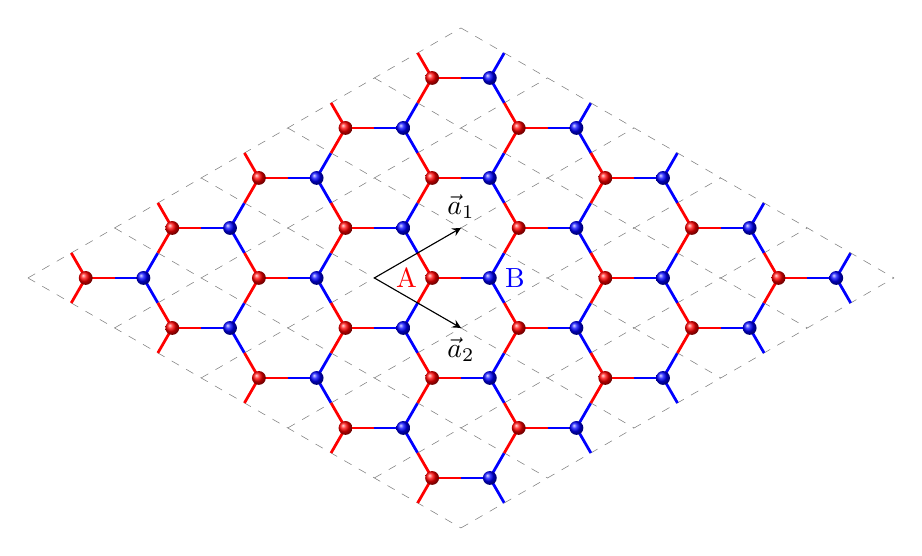
\begin{tikzpicture}
  [x=0.5in, y=0.5in]
  % define the basis vectors
  \coordinate (A1) at ({sqrt(3)/2}, 0.5);
  \coordinate (A2) at ({sqrt(3)/2},-0.5);
  \coordinate (b1) at ({  sqrt(3)/3}, 0.0);
  \coordinate (b2) at ({2*sqrt(3)/3}, 0.0);

  % plot the lattice and grid point
  \foreach \ii in {0,...,5}{
    \foreach \jj in {0,...,5}{
      \ifthenelse{\ii=0}{
        \draw[help lines, dashed] ($ \jj *(A2) $) -- ++($ 5 *(A1) $);
      }{}
      \ifthenelse{\jj=0}{
        \draw[help lines, dashed] ($ \ii *(A1) $) -- ++($ 5 *(A2) $);
      }{}

      \ifthenelse{\ii<5 \and \jj<5}{
        \foreach \kk in {0, 1, 2}{
          \draw[red , line width=1] ($ \ii *(A1) + \jj *(A2) + (b1) $)-- ++(\kk*120:{sqrt(3)/6});
          \draw[blue, line width=1] ($ \ii *(A1) + \jj *(A2) + (b2) $)-- ++(\kk*120+60:{sqrt(3)/6});
        }
        \shade[ball color=red ] ($ \ii *(A1) + \jj *(A2) + (b1) $) circle (2.5pt);
        \shade[ball color=blue] ($ \ii *(A1) + \jj *(A2) + (b2) $) circle (2.5pt);
      }{}
    }
  }

  \begin{scope}
    [shift={({2*sqrt(3)}, 0)}]
    \draw[<->, >=stealth, black] ({sqrt(3)/2}, 0.5) -- (0, 0)
        node[pos=0.0, above] {$\vec{a}_1$}
        -- ({sqrt(3)/2},-0.5)
        node[pos=1.0, below] {$\vec{a}_2$};
   ;
    \node[left=2pt] at ({  sqrt(3)/3}, 0.0) {\textcolor{red}{A}};
    \node[right=2pt] at ({2*sqrt(3)/3}, 0.0) {\textcolor{blue}{B}};
  \end{scope}

\end{tikzpicture}

\end{document}
